\chapter{Incorporación de Bases de Datos de Alta Resolución}
La utilización del modelo WRF con dominios anidados hasta resoluciones del orden de los metros, exige la implementación de bases de datos no nativas del software para la información estática (orografía y uso de suelo) en los dominios.

En este anexo se presenta el mapeo de las bases de datos descritas en las Tablas \ref{tab:05_caract_hov} y \ref{tab:05_caract_bol}, y una breve explicación acerca de cómo se manejaron las bases de datos.

Con respecto a la manipulación de los datos, esta se realizó a través un software GIS (\emph{Geographic Information System}) y la librería GDAL para la conversión de la extensión de los archivos. En particular, se utilizó el programa QGIS que es gratuito y de código libre. Los trabajos hechos incluyen:
\begin{itemize*}
	\item Conversión de los datos Corine (CLC12) al formato de clasificación USGS24 y su correspondiente transformación a formato binario.
	\item Transformación del datúm de la base de datos orográfica entregada por la campaña de medición de Bolund a WGS84.
	\item Creación de la base de datos para el uso de suelo en Bolund según lo declarado por la campaña \citep{3d4285ac04444eb3b9775baf9af052c6}.
	\item Refinamiento de los datos CLC12 (hecho de manera manual) para ajustar al contorno de la colina de Bolund.
	\item Ajuste de alturas de la base de datos orográfica de Bolund para su correcta implementación en WPS (fijar la altura de agua en $z=0$).
	\item Transformación de todos los datos a formato binario para la lectura del WPS.
\end{itemize*}

A continuación se presentan algunos ejemplos de códigos simples desarrollados para las tareas descritas.

Código en QGIS para la transformación de CLC12 a USGS24 según \cite{Pineda2004}:
\lstset{style=consola}
\begin{lstlisting}
("test@1"<=11)*1+("test@1"=12)*2+("test@1"=13)*3+("test@1"=14)*3+
("test@1"=15)*6+("test@1"=16)*6+("test@1"=17)*6+("test@1"=18)*2+
("test@1"=19)*6+("test@1"=20)*6+("test@1"=21)*6+("test@1"=22)*6+
("test@1"=23)*11+("test@1"=24)*14+("test@1"=25)*15+("test@1"=26)*7+
("test@1"= 27)*9+("test@1"=28)*9+("test@1"=29)*9+("test@1"=30)*19+
("test@1"=31)*19+("test@1"=32)*19+("test@1"=33)*19+("test@1"=34)*24+
("test@1"=35)*17+("test@1"=36)*17+("test@1"=37)*17+("test@1"=38)*17+
("test@1"=39)*17+("test@1"=40)*16+("test@1"=41)*16+("test@1"=42)*16+
("test@1"=43)*16+("test@1">=44)*16
\end{lstlisting}
Código GDAL para la generación de uso de suelo en Bolund a partir de su orografía:
\begin{lstlisting}
gdal_calc.py -A bolund_rought_displaced_wgs84.tif --outfile=result.tif 
--calc="16*(A<0.01)+2*(A>0.01)"
\end{lstlisting}
Código GDAL para la conversión del uso de suelo de Bolund de GeoTIFF a binario:
\begin{lstlisting}
gdal_translate -of ENVI -ot Int16 result.tif BOLUND_LANDUSE.bil
\end{lstlisting}
Código GDAL para correjir los valores indefinidos generados por la rotación del datúm:
\begin{lstlisting}
gdal_calc.py -A BOLUND_LANDUSE.bil --outfile=BOLUND_LANDUSE2.bil 
--calc="(A==32767)*16+(A<32767)*A"
\end{lstlisting}

Finalmente las bases de datos introducidas de orografía y uso de suelo se ven en el modelo como las Figuras \ref{fig:dominios_hov} y \ref{fig:dominios_bol}. Notar que el color amarillo para la categoría de uso de suelo significa la incorporación manual del $z_0$ según la información presente en las publicaciones correspondientes para cada dominio.
\newpage
\vspace*{\fill}
\begin{figure}[H]
	\centering
	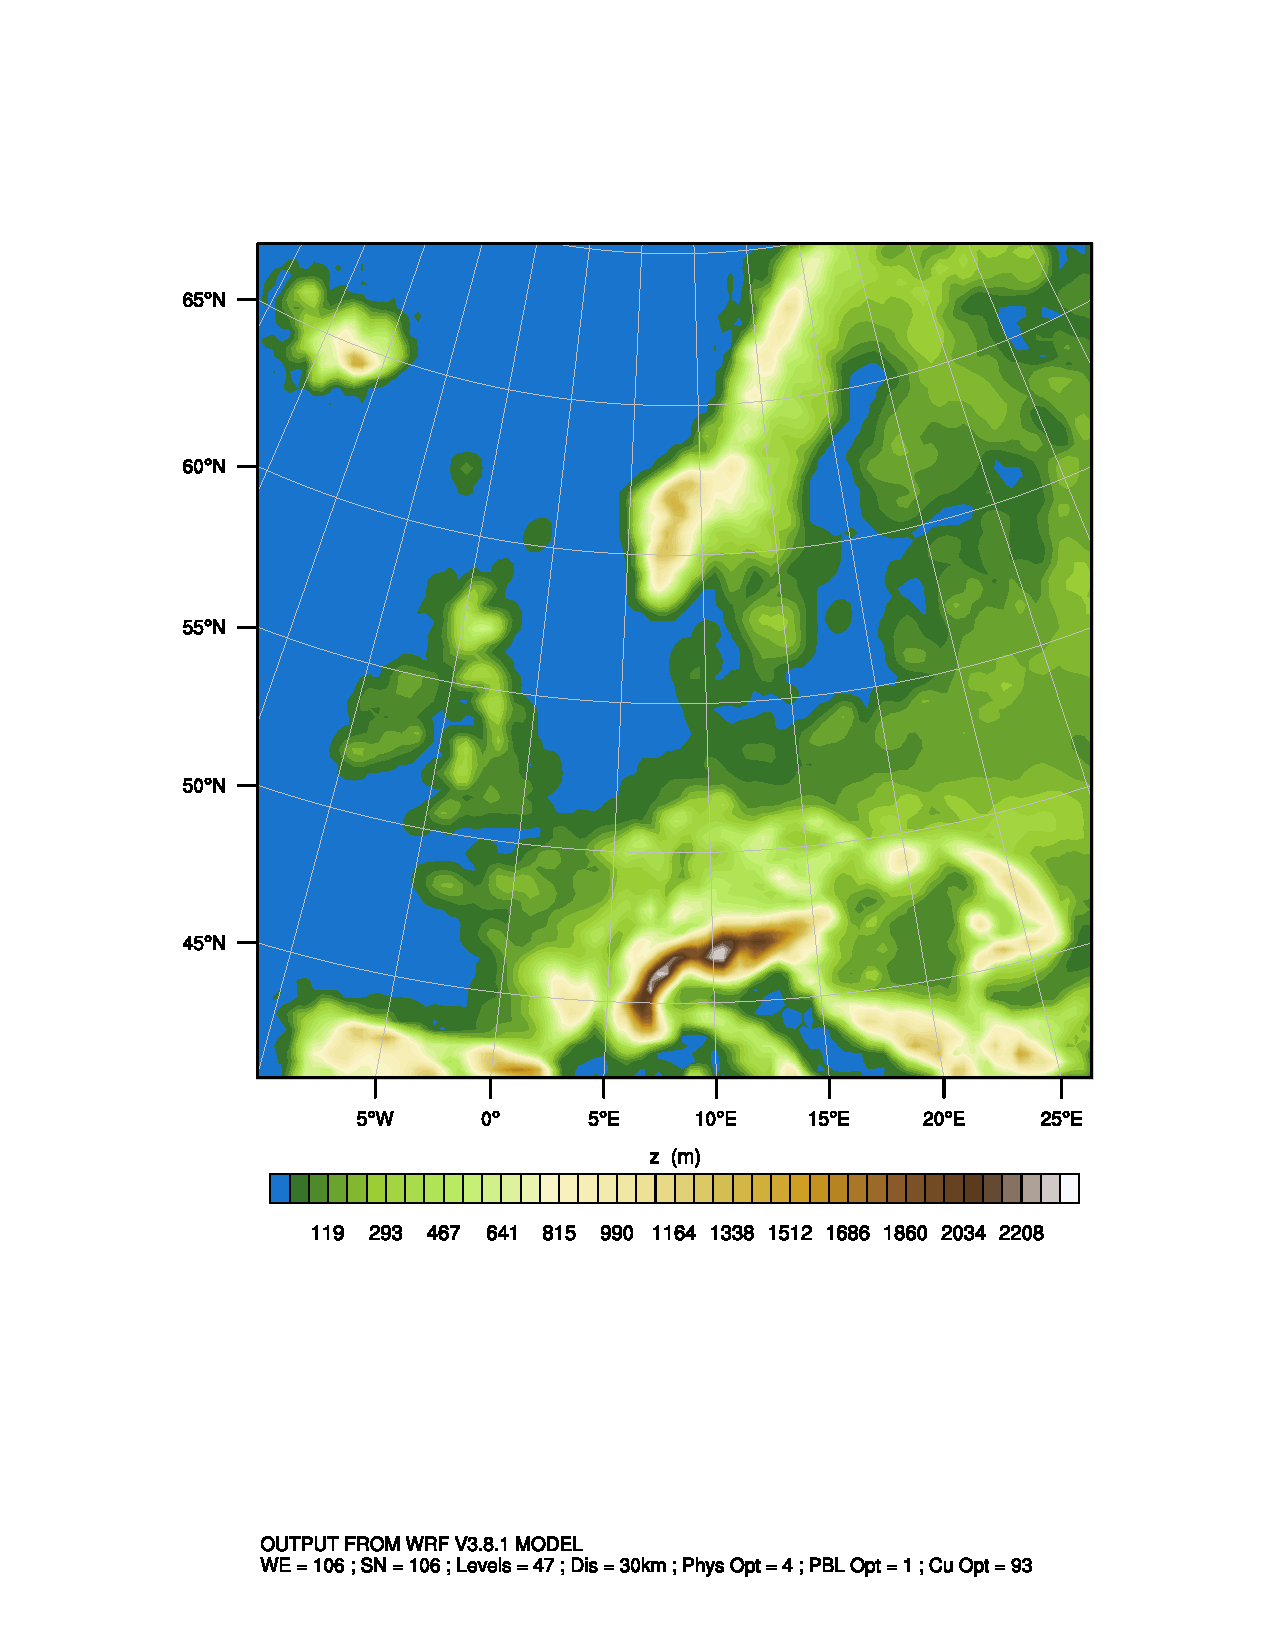
\includegraphics[width=0.25\linewidth,page=1,trim={2cm 6.5cm 1cm 3.5cm},clip]{Imagenes/05/hov_domain.pdf}%
	\includegraphics[width=0.25\linewidth,page=2,trim={2cm 6.5cm 1cm 3.5cm},clip]{Imagenes/05/hov_domain.pdf}%
	\includegraphics[width=0.25\linewidth,page=3,trim={2cm 6.5cm 1cm 3.5cm},clip]{Imagenes/05/hov_domain.pdf}%
	\includegraphics[width=0.25\linewidth,page=4,trim={2cm 6.5cm 1cm 3.5cm},clip]{Imagenes/05/hov_domain.pdf}%
	
	\bigskip
	\includegraphics[width=0.25\linewidth,page=5,trim={2cm 6.5cm 1cm 3.5cm},clip]{Imagenes/05/hov_domain.pdf}%
	\includegraphics[width=0.25\linewidth,page=6,trim={2cm 6.5cm 1cm 3.5cm},clip]{Imagenes/05/hov_domain.pdf}%
	\includegraphics[width=0.25\linewidth,page=7,trim={2cm 6.5cm 1cm 3.5cm},clip]{Imagenes/05/hov_domain.pdf}%
	\includegraphics[width=0.25\linewidth,page=8,trim={2cm 6.5cm 1cm 3.5cm},clip]{Imagenes/05/hov_domain.pdf}%
	
	\bigskip
	\includegraphics[width=0.25\linewidth,page=9,trim={2cm 6.5cm 1cm 3.5cm},clip]{Imagenes/05/hov_domain.pdf}%
	\includegraphics[width=0.25\linewidth,page=10,trim={2cm 6.5cm 1cm 3.5cm},clip]{Imagenes/05/hov_domain.pdf}%
	\includegraphics[width=0.25\linewidth,page=11,trim={2cm 6.5cm 1cm 3.5cm},clip]{Imagenes/05/hov_domain.pdf}%
	\includegraphics[width=0.25\linewidth,page=12,trim={2cm 6.5cm 1cm 3.5cm},clip]{Imagenes/05/hov_domain.pdf}%
	
	\bigskip
	\includegraphics[width=0.25\linewidth,page=13,trim={2cm 6.5cm 1cm 3.5cm},clip]{Imagenes/05/hov_domain.pdf}%
	\includegraphics[width=0.25\linewidth,page=14,trim={2cm 6.5cm 1cm 3.5cm},clip]{Imagenes/05/hov_domain.pdf}%
	
	\caption{Orografía (MSNM) y uso de suelo (categoría USGS24) de alta resolución para cada uno de las mallas anidadas (d01-d07) en Høvsøre.}
	\label{fig:dominios_hov}
\end{figure}
\vspace*{\fill}
\newpage
\vspace*{\fill}
\begin{figure}[H]
	\centering
	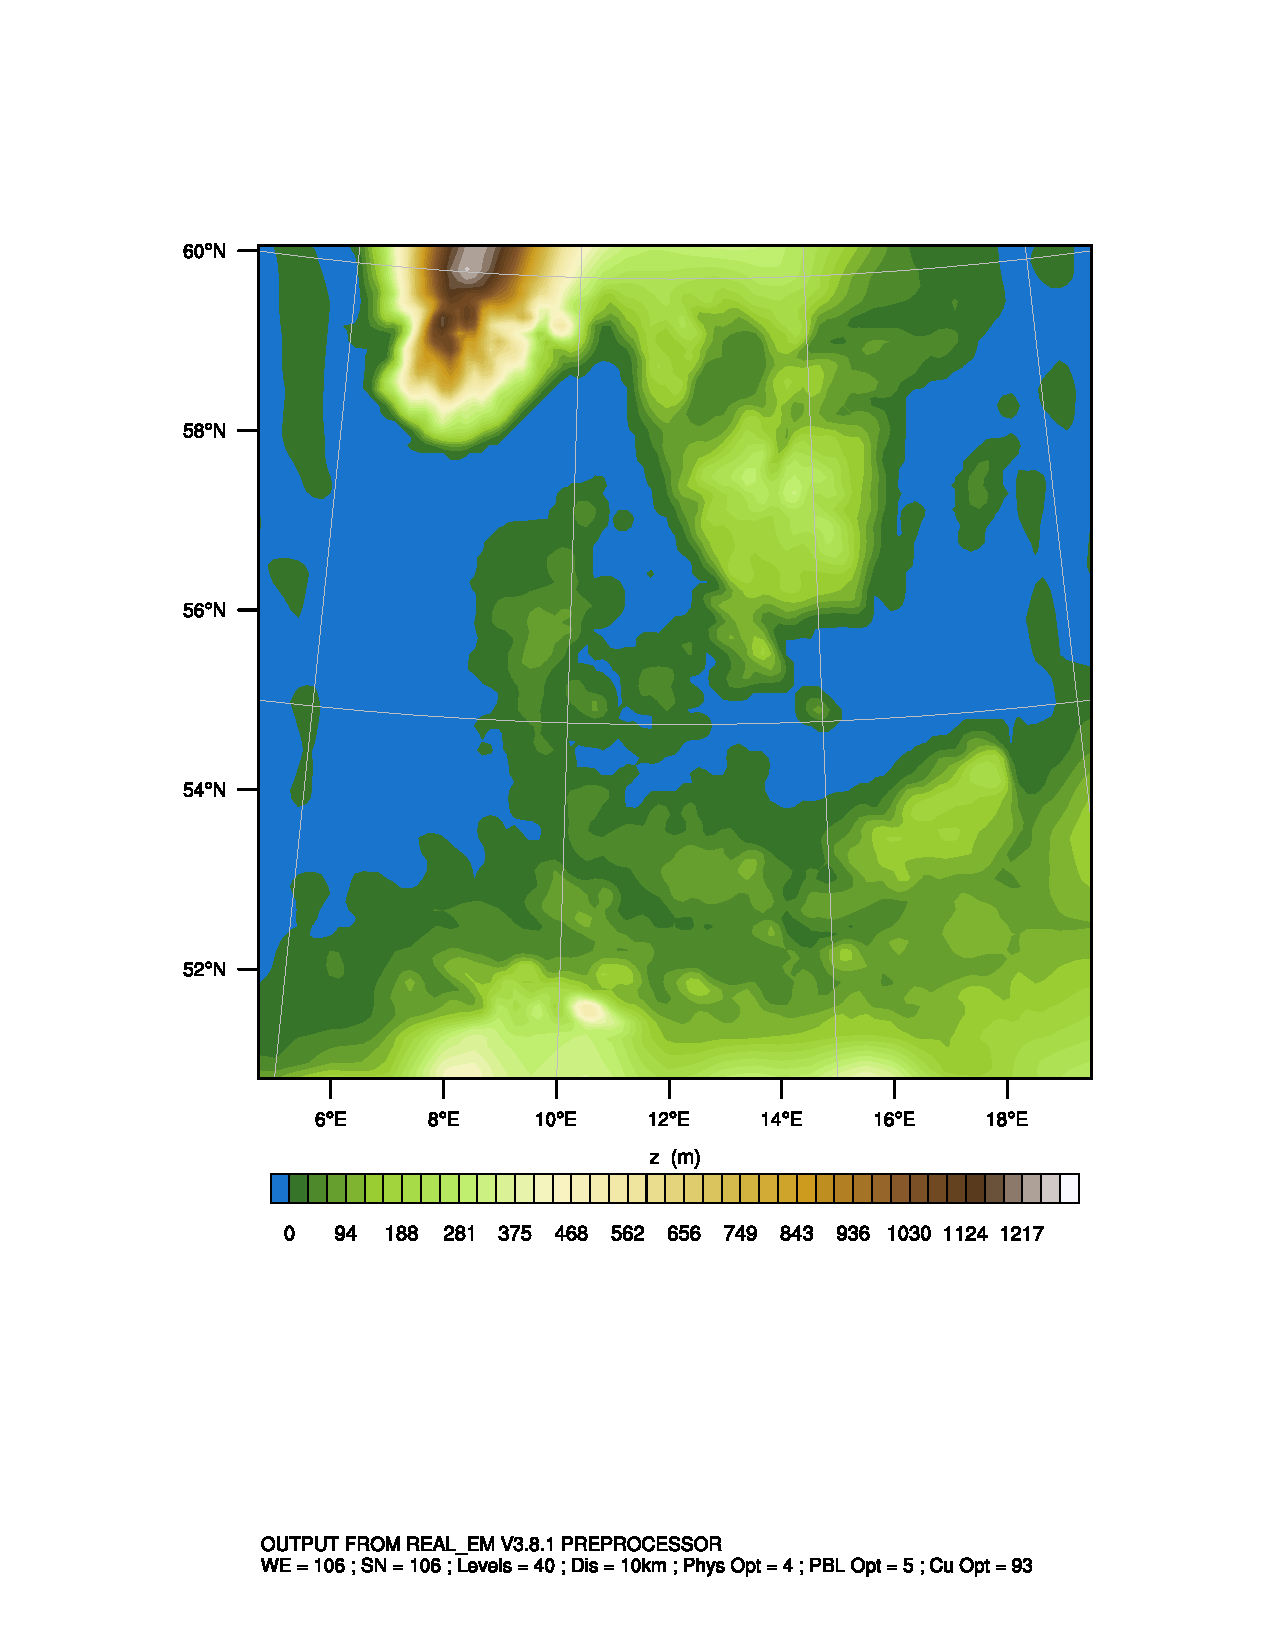
\includegraphics[width=0.25\linewidth,page=1,trim={2cm 6.5cm 1cm 3.5cm},clip]{Imagenes/05/bol_domain.pdf}%
	\includegraphics[width=0.25\linewidth,page=2,trim={2cm 6.5cm 1cm 3.5cm},clip]{Imagenes/05/bol_domain.pdf}%
	\includegraphics[width=0.25\linewidth,page=3,trim={2cm 6.5cm 1cm 3.5cm},clip]{Imagenes/05/bol_domain.pdf}%
	\includegraphics[width=0.25\linewidth,page=4,trim={2cm 6.5cm 1cm 3.5cm},clip]{Imagenes/05/bol_domain.pdf}%
	
	\bigskip
	\includegraphics[width=0.25\linewidth,page=5,trim={2cm 6.5cm 1cm 3.5cm},clip]{Imagenes/05/bol_domain.pdf}%
	\includegraphics[width=0.25\linewidth,page=6,trim={2cm 6.5cm 1cm 3.5cm},clip]{Imagenes/05/bol_domain.pdf}%
	\includegraphics[width=0.25\linewidth,page=7,trim={2cm 6.5cm 1cm 3.5cm},clip]{Imagenes/05/bol_domain.pdf}%
	\includegraphics[width=0.25\linewidth,page=8,trim={2cm 6.5cm 1cm 3.5cm},clip]{Imagenes/05/bol_domain.pdf}%
	
	\bigskip
	\includegraphics[width=0.25\linewidth,page=9,trim={2cm 6.5cm 1cm 3.5cm},clip]{Imagenes/05/bol_domain.pdf}%
	\includegraphics[width=0.25\linewidth,page=10,trim={2cm 6.5cm 1cm 3.5cm},clip]{Imagenes/05/bol_domain.pdf}%
	\includegraphics[width=0.25\linewidth,page=11,trim={2cm 6.5cm 1cm 3.5cm},clip]{Imagenes/05/bol_domain.pdf}%
	\includegraphics[width=0.25\linewidth,page=12,trim={2cm 6.5cm 1cm 3.5cm},clip]{Imagenes/05/bol_domain.pdf}%
	
	\bigskip
	\includegraphics[width=0.25\linewidth,page=13,trim={2cm 6.5cm 1cm 3.5cm},clip]{Imagenes/05/bol_domain.pdf}%
	\includegraphics[width=0.25\linewidth,page=14,trim={2cm 6.5cm 1cm 3.5cm},clip]{Imagenes/05/bol_domain.pdf}%
	
	\bigskip
	\includegraphics[width=0.25\linewidth,page=15,trim={0cm 6.5cm 1cm 3.5cm},clip]{Imagenes/05/bol_domain.pdf}%
	\includegraphics[width=0.25\linewidth,page=16,trim={0cm 6.5cm 1cm 3.5cm},clip]{Imagenes/05/bol_domain.pdf}%
	
	\caption{Orografía (MSNM) y uso de suelo (categoría USGS24) de alta resolución para cada uno de las mallas anidadas (d01-d08) en Bolund.}
	\label{fig:dominios_bol}
\end{figure}
\vspace*{\fill}
